\chapter[Governança]{Governança}
\label{governanca}

Neste capítulo iremos abordar a teoria geral da administração que deu origem 
ao modo de administrar que conhecemos hoje, conceitos de governança e o modo 
como a governo federal desenvolve software embasado no Processo de Software
do SISP.

\section{Teoria Geral da Administração}

A preocupação em racionalizar, padronizar e prescrever normas é estudada desde a 
Administração Científica proposta por Taylor. Segundo essa proposta a gerência 
deve seguir 4 princípios~\cite{chiavenato2001teoria}:

\begin{enumerate}
\item Princípio de planejamento. Substituir no trabalho o critério individual 
do operário, a improvisação e a atuação empírico-prática, por métodos baseados 
em procedimentos científicos. Substituir a improvisação pela ciência através
do planejamento do método de trabalho.
 
\item Princípio de preparo. Selecionar científicamente os trabalhadores de acordo 
com suas aptidões e prepará-los e treiná-los para produzirem mais e melhor, de 
acordo com o método planejado. Preparar máquinas e equipamentos em um arranjo 
físico e disposição racional.

\item Princípio do controle. Controlar o trabalho para se certificar de que está 
sendo executado de acordo com os métodos estabelecidos e segundo o plano previsto. 
A gerência deve cooperar com os trabalhadores para que a execução seja a melhor 
possível.

\item Princípio da execução. Distribuir atribuições e responsabilidades para 
que a execução do trabalho seja disciplinada.
\end{enumerate}

A Administração científica deu pouca importância para os aspectos humanos de uma
organização, restringindo-se apenas a fatores relacionados diretamente com o 
cargo ou função do operário, embora saibamos que uma organização é constituída 
por pessoas.
%
Paralelamente ao surgimento da Administração Científica de Taylor surgia a 
Administração Clássica, que diferentemente da teoria de Taylor que se caracterizava
pela ênfase na tarefa realizada pelo operário, se caracterizava pela ênfase na 
estrutura da organização com o mesmo objetivo de buscar a eficiência das
organizações~\cite{chiavenato2001teoria}.

Na Teoria Clássica, preconizada por Fayol, ao contrário, partia-se do todo 
organizacional e da sua estrutura para garantir eficiência a todas as partes 
envolvidas, fossem elas órgãos (como seções, departamentos etc.) ou pessoas 
(como ocupantes de cargos e executores de tarefas).
%
Fayol define o ato de administrar como: prever, organizar, comandar, coordenar 
e controlar. As funções administrativas envolvem os elementos da Administração, 
isto é, as funções do administrador~\cite{chiavenato2001teoria}:

\begin{enumerate}

\item Prever. Visualizar o futuro e traçar o programa de ação.

\item Organizar. Constituir o duplo organismo material e social da empresa.

\item Comandar. Dirigir e orientar o pessoal.

\item Coordenar. Ligar, unir, harmonizar todos os atos e esforços coletivos.

\item Controlar. Verificar que tudo ocorra de acordo com as regras estabelecidas 
e as ordens dadas.

\end{enumerate}

Com o surgimento da Abordagem humanística e a Teoria das Relações Humanas,
a teoria Administrativa passa por uma revolução conceitual: a transferência da 
ênfase antes colocada na tarefa (pela Administração Científica) e na estrutura 
organizacional (pela Teoria Clássica) para a ênfase nas pessoas que trabalham 
ou que participam nas organizações. A Abordagem Humanística faz com que a
preocupação com a máquina e com o método de trabalho e a preocupação com a 
organização formal e os princípios de Administração cedam prioridade para a 
preocupação com as pessoas e os grupos sociais.


\section{Conceito de Governança}

Governança pode ser definida como o sistema pelo qual as organizações 
são monitoradas envolvendo o relacionamento entre todos os integrantes,
são recomendações objetivas alinhando interesses na intenção de preservar e 
otimizar o valor da organização, em outras palavras é um conjunto de processos
que regulam a maneira como uma organização é dirigida e estuda as relações entre 
os diferentes atores que a compõe.\cite{molinarogestao}

Mais especificamente para tecnologia da informação um sistema de governança
estabelece mecanismos, estruturas e incentivos, que compõem o sistema de controle de 
gestão da empresa e direciona o comportamento dos administradores para o cumprimento 
dos objetivos estipulados pelos acionistas/proprietários.\cite{martin2004governancca}
%
Segundo a Ministry of international trade and industry do MIT\footnote{http://www.mti.gov.bw/content/international-trade} 
Além de "Capacidade organizacional de controlar a formulação e implementação da 
estratégia de TI e guiar a mesma na direção adequada com o propósito de gerar 
vantagens competitivas para a corporação”

Governança de TI quando implantada de forma efetiva contribui para a melhora da 
performance, que por sua vez contribui para a melhora da organização como um todo
\cite{tres2014information}.

Os conjuntos de processos definidos pela governança visam além de organizar, 
dar transparência ao trabalho a ser realizado.
%
Processo é um conjunto seqüencial de ações baseado em estratégia para alcançar
um objetivo. Para definir uma estratégia são necessários 3 passos, identificar a
situação do ambiente, identificar a situação da organização e por fim é comparada
a situação do ambiente e da organização e identificados os cursos alternativos
de ação e escolhida a melhor alternativa~\cite{molinarogestao}.

Trazendo para a realidade do Novo Portal do Software público, a governança pode ser usada para 
definir um processo que auxilie na gestão do Portal como um todo, e mais especificamente,
das comunidades que nele estão contidas, imprimindo organização e controle para atender 
a demanda não somente do governo mas também dos usuários da nova plataforma.

Para que este desenho faça sentido é necessário que seja colocado no processo somente o que 
realmente tem valor de negócio para o usuário e para os gestores.

A definição da governaça dará subsídios para sejam notados os padrões de uso e colaboração na
nova plataforma, podendo assim ser geradas algumas "boas práticas" para uso e colaboração
visando a manutenebilidade da plataforma.

\section{Processo de Software para o SISP (PSW-SISP)}

O Sistema de Administração dos Recursos de Tecnologia da Informação – SISP, 
foi instituído pelo Decreto n 1.048 de 21 de janeiro de 1994\footnote{http://www.planalto.gov.br/ccivil\_03/decreto/1990-1994/D1048.htm}
e atualizado pelo Decreto n 7.579 de 11 de outubro de 2011\footnote{http://www.planalto.gov.br/ccivil\_03/\_Ato2011-2014/2011/Decreto/D7579.htm}, 
com o objetivo de organizar a operação, 
controle, supervisão e coordenação dos recursos de informação e informática da 
administração direta, autárquica e fundacional do Poder Executivo Federal, sendo 
facultada às empresas públicas e às sociedades de economia mista a participação no SISP, 
cujas condições devem constar de termo próprio a ser firmado entre os dirigentes das 
entidades e o titular do Órgão Central do SISP\footnote{http://www.sisp.gov.br/}.

O processo de software para o SISP aborda as atividades ligadas ao desenvolvimento 
e as atividades ligadas ao planejamento de recursos para o ambiente necessário para
o software.
\newpage
\begin{figure}[htpb]
 \begin{center}
    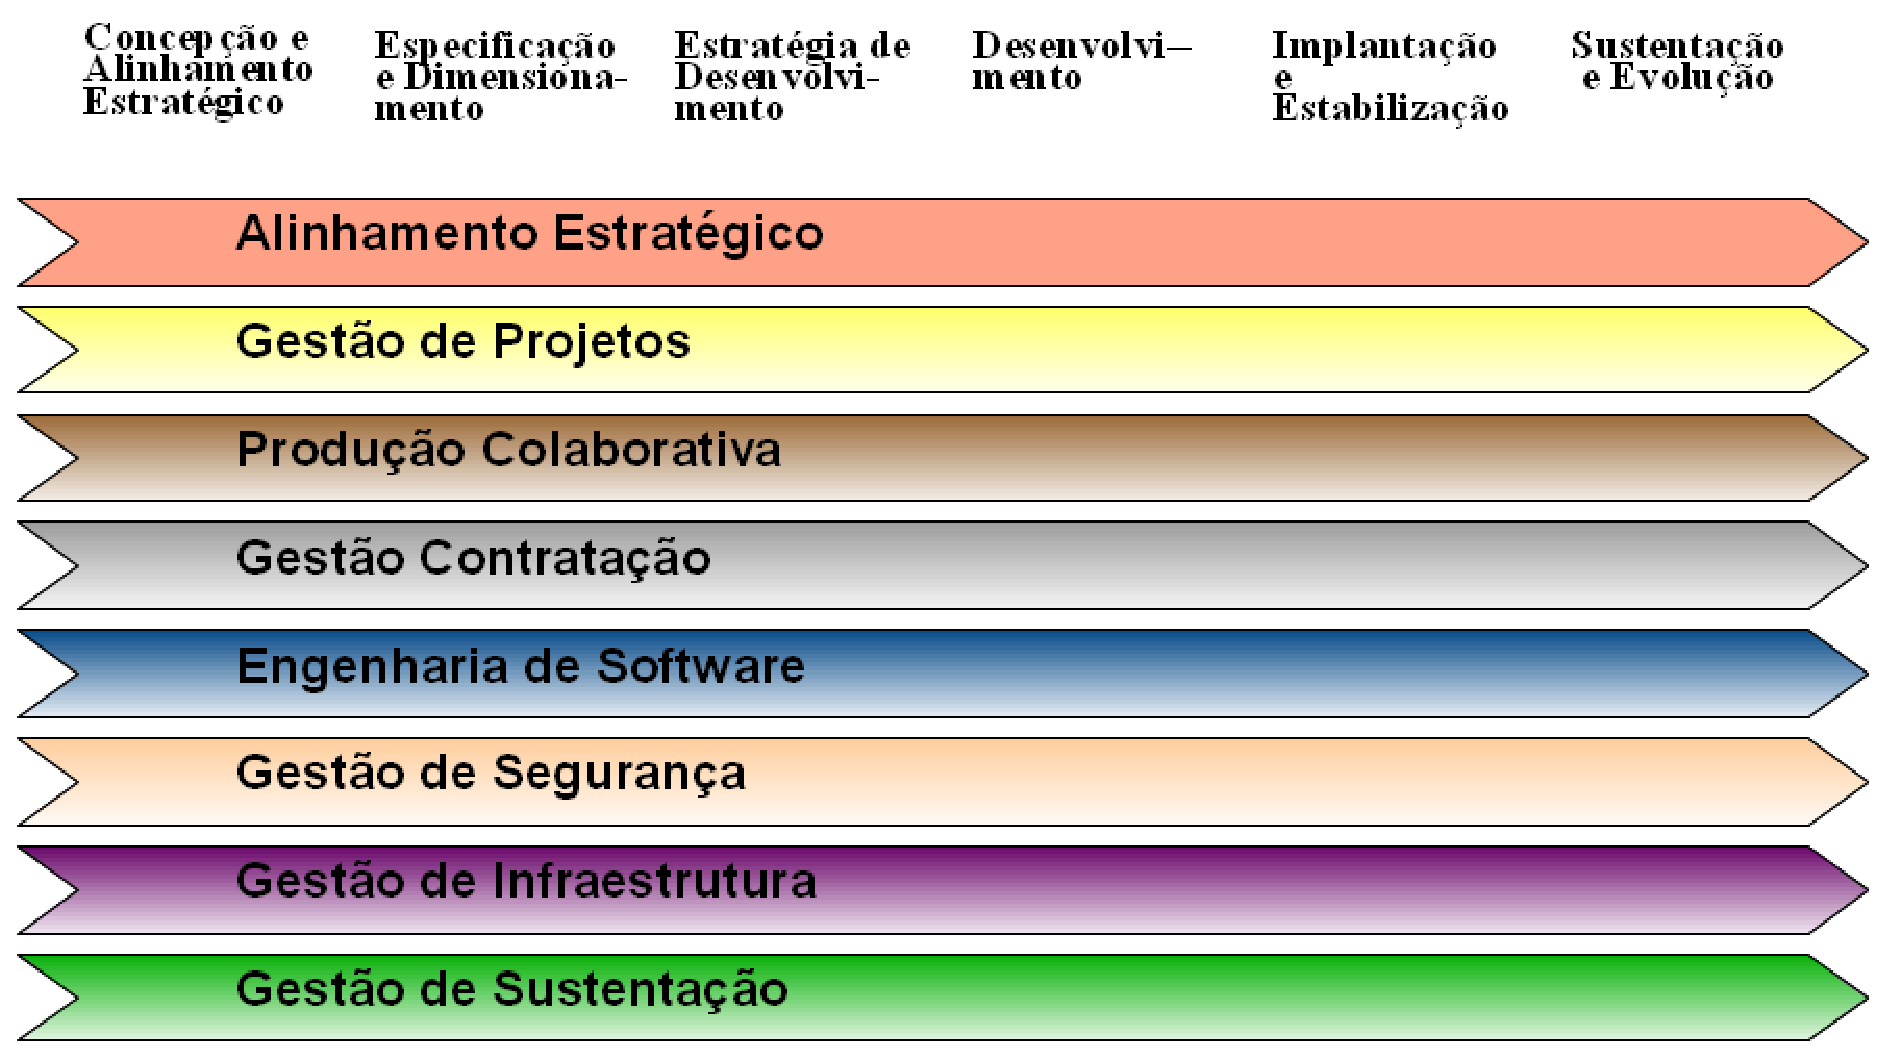
\includegraphics[width=.90\textwidth]{figuras/EstruturaPSW.eps}
 \end{center}
  \caption{Processo de software para o SISP(PSW-SISP)}
  \label{fig:core_concurrent}
\end{figure}

O processo é dividido em 6 fases:

\begin{itemize}
\item Concepção e Alinhamento estratégico: Esta fase inicia com o envio do 
documento de oficialização da demanda (DOD) da Área Requisitante para a Área de 
TI, que irá verificar o alinhamento estratégico da demanda com os instrumentos 
estratégicos do órgão e, caso não esteja alinhada, irá devolver o DOD à Área 
Requisitante para que, após a estimativa de custo preliminar do projeto de software 
realizado pela Área de TI, a mesma solicite a mudança do PDTI ao Comitê de TI. O 
comitê de TI irá analisar a possibilidade de incluir a demanda não planejada e, 
caso seja viável, atualizará o PDTI. Caso esteja alinhado estrategicamente, a 
Área de TI irá elaborar o termo de abertura e iniciar o projeto;(PSW-SISP)

\item Especificação e dimensionamento: Esta fase destina-se ao entendimento e 
dimensionamento da demanda de software através da definição do escopo do produto, 
da modelagem de negócio e do levantamento dos requisitos funcionais e não funcionais;
(PSW-SISP)

\item Estratégia de desenvolvimento:Essa fase destina-se a escolher a estratégia 
de desenvolvimento (desenvolvimento interno, produção colaborativa ou contratação) 
mais adequada para o desenvolvimento e/ou manutenção do software (evolutiva, 
corretiva e adaptativa). Após escolhida a estratégia de desenvolvimento, será 
avaliado qual a melhor metodologia de desenvolvimento de sistemas e qual a infraestrutura 
e sustentação necessários para que o software funcione corretamente no ambiente de produção; 
(PSW-SISP)

\item Desenvolvimento: É a fase onde é iniciada a execução do projeto de acordo 
com o que foi planejado nas fases anteriores. O planejamento será atualizado 
sempre que necessário para se adequar às novas realidades de tempo, escopo, 
custo, qualidade e negócio; (PSW-SISP)

\item Implantação e Estabilização: Implantação do software (adequado ou desenvolvido) 
em seu ambiente de produção, para o seu uso efetivo, estabilizando a solução de 
acordo com o ambiente de execução e o retorno dos usuários; (PSW-SISP)

\item Sustentação e Evolução: manutenção da saúde do sistema (incluindo, mas não 
limitado à processos de backup de dados, segurança de acesso e outros), o suporte 
continuado aos usuários e o atendimento de novos requisitos que surgem do próprio 
uso e mudanças de processos no negócio. (PSW-SISP)

\end{itemize}

O processo possui ainda, oito eixos de trabalho que permeiam todas as fases:

\begin{itemize}

\item Alinhamento estratégico: Alinhamento da necessidade do software com as
necessidades de negócio do órgão descritas nos seus instrumentos estratégicos;

\item Gestão de projetos: Os processos de gestão de projetos serão mapeados 
tendo como referência a Metodologia de Gerenciamento de Projetos do SISP (MGP-SISP);

\item Produção Colaborativa: Desenvolvimento conjunto de software, ou seja, processos
que promovam o levantamento de requisitos comuns a mais de um órgão para que 
possam desenvolver ou contratar um software colaborativamente;

\item Gestão de Contratação: Conjunto de boas práticas para contratações de
soluções de TI. Os processos da gestão de contratação serão baseados e alinhados 
com a instrução normativa IN MP/SLTI no 04/2010 e no Manual de Contratações de 
Soluções de Tecnologia da Informação;

\item Engenharia de Software: Desenvolvimento e manutenção de sistemas baseado nas
melhores práticas difundidas no mercado e na literatura, e em metodologias 
utilizadas por órgãos e entidades da Administração Pública Federal;

\item Gestão da Segurança: Desenvolvimento seguro de software que envolve tanto a
segurança do ambiente de desenvolvimento quanto da aplicação desenvolvida;

\item Gestão da Infraestrutura: Construir um ambiente que tenha a capacidade 
necessária para prover serviços e uma estrutura adequada ao desenvolvimento de
software;

\item Gestão da Sustentação: Planejamento das condições necessárias para que o 
software desenvolvido seja mantido, operado e evoluído de forma sustentável e 
viável.
  	
\end{itemize}

Segundo o PSW-SISP, o intuito do processo é que ele seja usado conforme as 
necessidades e maturidade do órgão. Ficará a cargo dos órgãos decidir quais 
as atividades são adequadas à maturidade e ao projeto em desenvolvimento ou 
manutenção (corretiva, adaptativa e corretiva), sendo que algumas atividades 
mínimas são consideradas essenciais para a qualidade do software.
	






